\documentclass[11pt]{article}
\usepackage[scale=0.75,twoside,bindingoffset=5mm,a4paper]{geometry}
\usepackage[utf8]{inputenc}
\usepackage{kotex}
\usepackage{lmodern}
\usepackage{cite}
\usepackage{minted}
\usepackage{graphicx}

\author{20193601 지준섭}
\title{HeyMoney: Automatic Debt Management System With Messenger Conversation \\
\begin{large}
  CS579 Homework\#5: extended proposal
\end{large}}

\begin{document}

\maketitle


\section{Introduction}

While a person to a group, such as a circle, a laboratory, or a company,
there is always a problem of financial relationship.
The problem can be about a food eaten together,
a product purchased on behalf of another, or other important one.
Building a system that saves these financial records,
and shows summary would be useful.
But in that case, users must learn how to register the records.
So it would be much easier if we build a system that
automatically extracts financial information from the conversation in the messenger.

\section{Details}

\subsection{Requirements}

\begin{enumerate}
  \item The system should see whether the messsage is about money or not.
  \item The system should extract the amount of money from the message,
    and calculate results for each person.
  \item The system should notice which word is the people's name, and assign proper money to each person mentioned in the message.
  \item The system must cover \textit{Slack}, transactions database, and the webpage.
    To achieve this, the system must have an ability to send/receive HTTP request.
    The database must be set up to provide creditable records.
\end{enumerate}

\subsection{Structure}

Figure \ref{fig:diagram} briefly represents the structure of our system \textit{HeyMoney}.

\begin{figure}[!htbp]
  \centering
  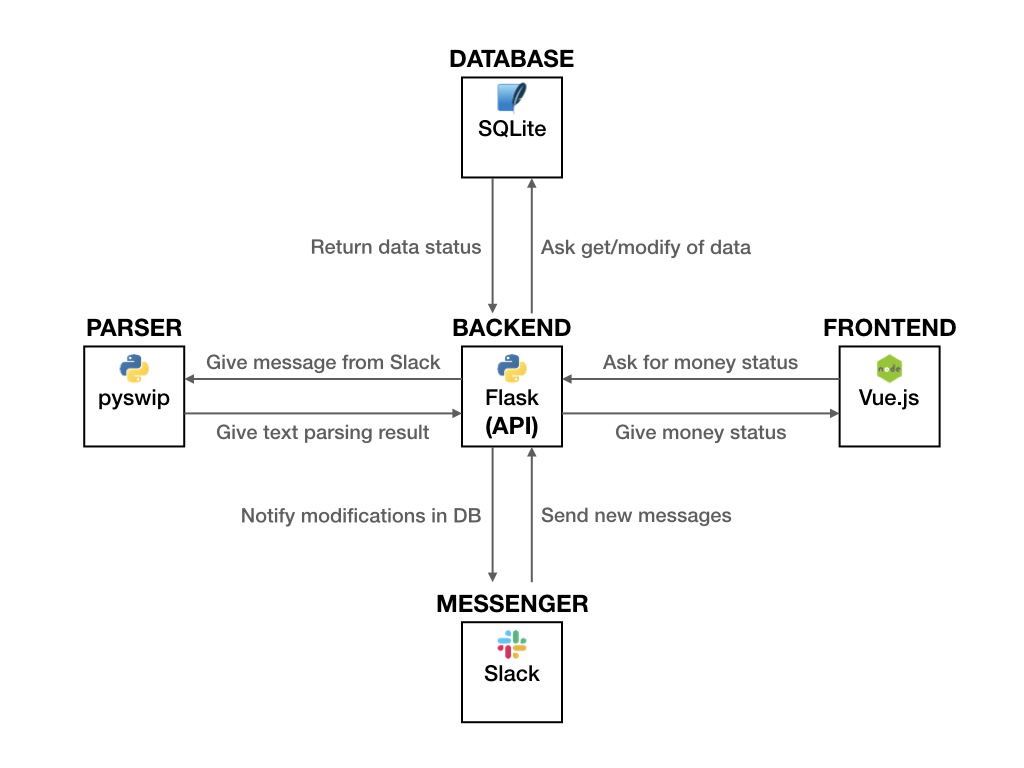
\includegraphics[width=\textwidth]{images/cl-hw3-diagram.png}
  \caption{The diagram of \textit{HeyMoney} system.}
  \label{fig:diagram}
\end{figure}

\subsubsection{Messenger -- \textit{Slack}}

For the project, we have to select a particular messenger for the development.
The messenger should satisfy these conditions:
\textbf{1.} should be widespread --
the system will become more useful when the more people use the messenger.
\textbf{2.} must provide an API and documents;
This feature makes us easy to debug and add functionalities.
So we choosed a \textit{Slack} to play a role of messenger.
\textit{Slack} is a widely-known for groups,
such as circles, laboratories, and companies.
It provides an official API and documentation
for accessing the messages in the channel,
so people can easily build a bot when they need a special function.

\subsubsection{Parser -- \textit{pyswip}}
Our system will receive the \textit{Slack} messages as input.
The message will have some attributes -- a \textit{username}, a \textit{timestamp},
and a \textit{body text}.
The \textit{username} is an unique id for the user,
the \textit{timestamp} represents a time the message sended,
and the \textit{body text} is in natural language form,
and parsing this feature will be our main challenge of the project.

The parser will extract the information such as
\textit{who(debtor) should give creditor a money}, and \textit{the amount of money}.
To do this, we will use a concept of Definite Clause Grammar(DCG), and customize it.
For example, let's think about some sentences,
\textit{``@John and @Mia should give me 3 dollars.''},
and \textit{``I gave @Mike 3 dollars''}.
With DCG, we can extract some noun phrases like
\textit{@John and @Mia}, \textit{me}, \textit{I}, and \textit{@Mike}.
They are noun phrases, and \textit{me} \& \textit{I} are especially pronouns.
In these sentences, we can assume that the pronouns mean the sender of the message.
Also, we can extract the amount of money like \textit{3 dollars}.
Then the sentences can be represented like \textit{`debt([john, mia], Sender, 3)'},
and \textit{`pay(Sender, [mike], 3)'}. And these representations will
make the database add a debt/pay log.

Thanks to the broad communities of the language \textit{Python},
we could find a library \textit{pyswip},
which can process the same function as \textit{SWI-Prolog} in Python environment.
With this, the parser will receive the data(message) from the backend directly
and decide whether the message should make debt log or payment log.

\subsubsection{Backend -- \textit{Flask}}
The backend server plays most of the role in this system.
It should communicate with four other parts of the system:
the messenger, the parser, the database, and the frontend server.
With the messenger, it receives new messages from messenger,
and send results of the DB modification(notifications) to the messenger.
With the parser, it sends the data(message) to the parser,
and receives the parsed result.
If the parsed result is valid, the backend should interact with database.
It sends the request of modifying the data to the database,
and get a result of request.
Sometimes the frontend server makes an API call to get the status of the debt,
such as a summarization, or statistics.
Then the backend will make some requests of getting data, process it, and send the result back.
To achieve these features, we selected Flask as a Python library,
because it enables an effective develpment and a big extensibility.

\subsubsection{Database -- \textit{SQLite}}
The database saves all the logs of debt and payment.
When the request originally from the frontend server arrives, the database
will calculate the stats based on the query and return the result.
When the request is from the parser, the database will add a row to the
debt or the pay collection.
The new row should include the debtor and creditor, amount of debt,
and the time when the message was sent.
We choose \textit{SQLite} as the database of the system,
because it allows us easier data management with just one file.

\subsubsection{Frontend -- \textit{Vue.js}}
User must want to see their debt status in a readable form.
The frontend server is a solution for this demand.
The server send database a request to get the statistics through the backend,
and represent the result in a readable form: such as tables and graphs.
The components can be about total statistics of the group, or about a user.
\textit{Vue.js}, a library of \textit{Node.js} will just fit for this performance.
The library requires less communication with the backend server,
so it is easy to optimize the speed of the application.
Also, there is a lot of graph modules can be attached to the \textit{Vue.js}.


\subsection{Scenario}
\subsubsection{The user requests money to other people}
For example, a user buys a dinner to eat with two people together,
and want to ask for a money.
The user can say ``@John and @Mia, give me total 20,000 won for a dinner.'',
or ``@John and @Mia, Give me 10,000 won each.''.
The system should analyze both kinds of request,
and assign a proper amount of money to the people.
Both sentences will be represented as \textit{`debt([john, mia], Sender, 10000)'},
and the debt log will be added to the database.

\subsubsection{The user wants a notice that he/she has paid the debt}
After sending a proper money to the creditor,
the debtor will say ``I just sent 10,000 won to @Mike and @Amy.'', 
This sentence can be represented as \textit{`pay(Sender, [Mike, Amy], 10000)'}.
Before adding the payment log to the database, our system must check that
the sender really has the same or over 10,000 won debt to Mike and Amy.

\subsubsection{The user wants to view the debt summary}
In this case the user should access the web application.
The webpage should show the summary of debt/receivables,
and detailed information of each transaction, such as date, amount, item, and person.


\section{Progress}

\subsection{Done Works}
\begin{itemize}
  \item Creating a custom \textit{Slack} server
  \item Generating an API key to the \textit{Slack} server
  \item Building python-slack interface and receiving the message from the Slack
\end{itemize}

\subsection{Remaining Works}
\begin{itemize}
  \item Building a parser to extract the information from the message
  \item Desigining a web page for summarization
  \item Determining URL rule for the web app
  \item Database setup
  \item Building database-python interface
  \item Implementing REST API with Flask
\end{itemize}

\end{document}